%%__________________________________________________________________||
\section{Results}
\label{sec:interpretation}

A likelihood model of the observations in all data samples is used to
obtain a consistent prediction of the SM backgrounds and to test for
the presence of a variety of signal models.  In each bin of \scalht
for events in the same category of \njet and \nb, the observation is
modelled as a Poisson-distributed variable around the sum of the SM
expectation and a potential signal contribution (assumed to be zero in
the following discussion). The SM expectation is related to the
expected yields in the \mj, \mmj, and \gj control samples via transfer
factors derived from simulation. Likelihood functions describe the
yields in the \scalht bins of the \mj, \mmj, and \gj control samples
in the same category of \njet and \nb as the signal region. The
systematic uncertainties summarised in Table~\ref{tab:bkgd_systs} are
accommodated in the likelihood function by nuisance parameters, the
measurements of which are assumed to follow a log-normal
distribution. In the presence of a non-zero signal contribution, the
CL$_{\mathrm{s}}$ technique~\cite{read, Cowan:2010js} is used to
determine upper limits on production cross section using asymptotic
formulae.

The expected number of events from SM processes is determined from a
simultaneous fit to the signal region and up to three control
samples. The likelihood function is maximised over all fit parameters
under the SM-only hypothesis.
Figures~\ref{fig:mono}--\ref{fig:sym}
summarise the observed yields and ``pre-fit'' and ``post-fit'' SM
expectations for signal candidate events in the monojet, asymmetric,
and symmetric categories, respectively. No significant tension is
observed between the predictions and data in the signal region, which
is well described by the SM-only hypothesis.

Figure~\ref{fig:mht-templates} shows distributions of observed counts
in data and also expected counts from SM background processes, as a
function of the \mht variable for two \nb categories at high \njet and
\scalht, which are expected to provide sensitivity to models with
TeV-scale gluinos. 

\begin{figure}[!h]
  \begin{center}
    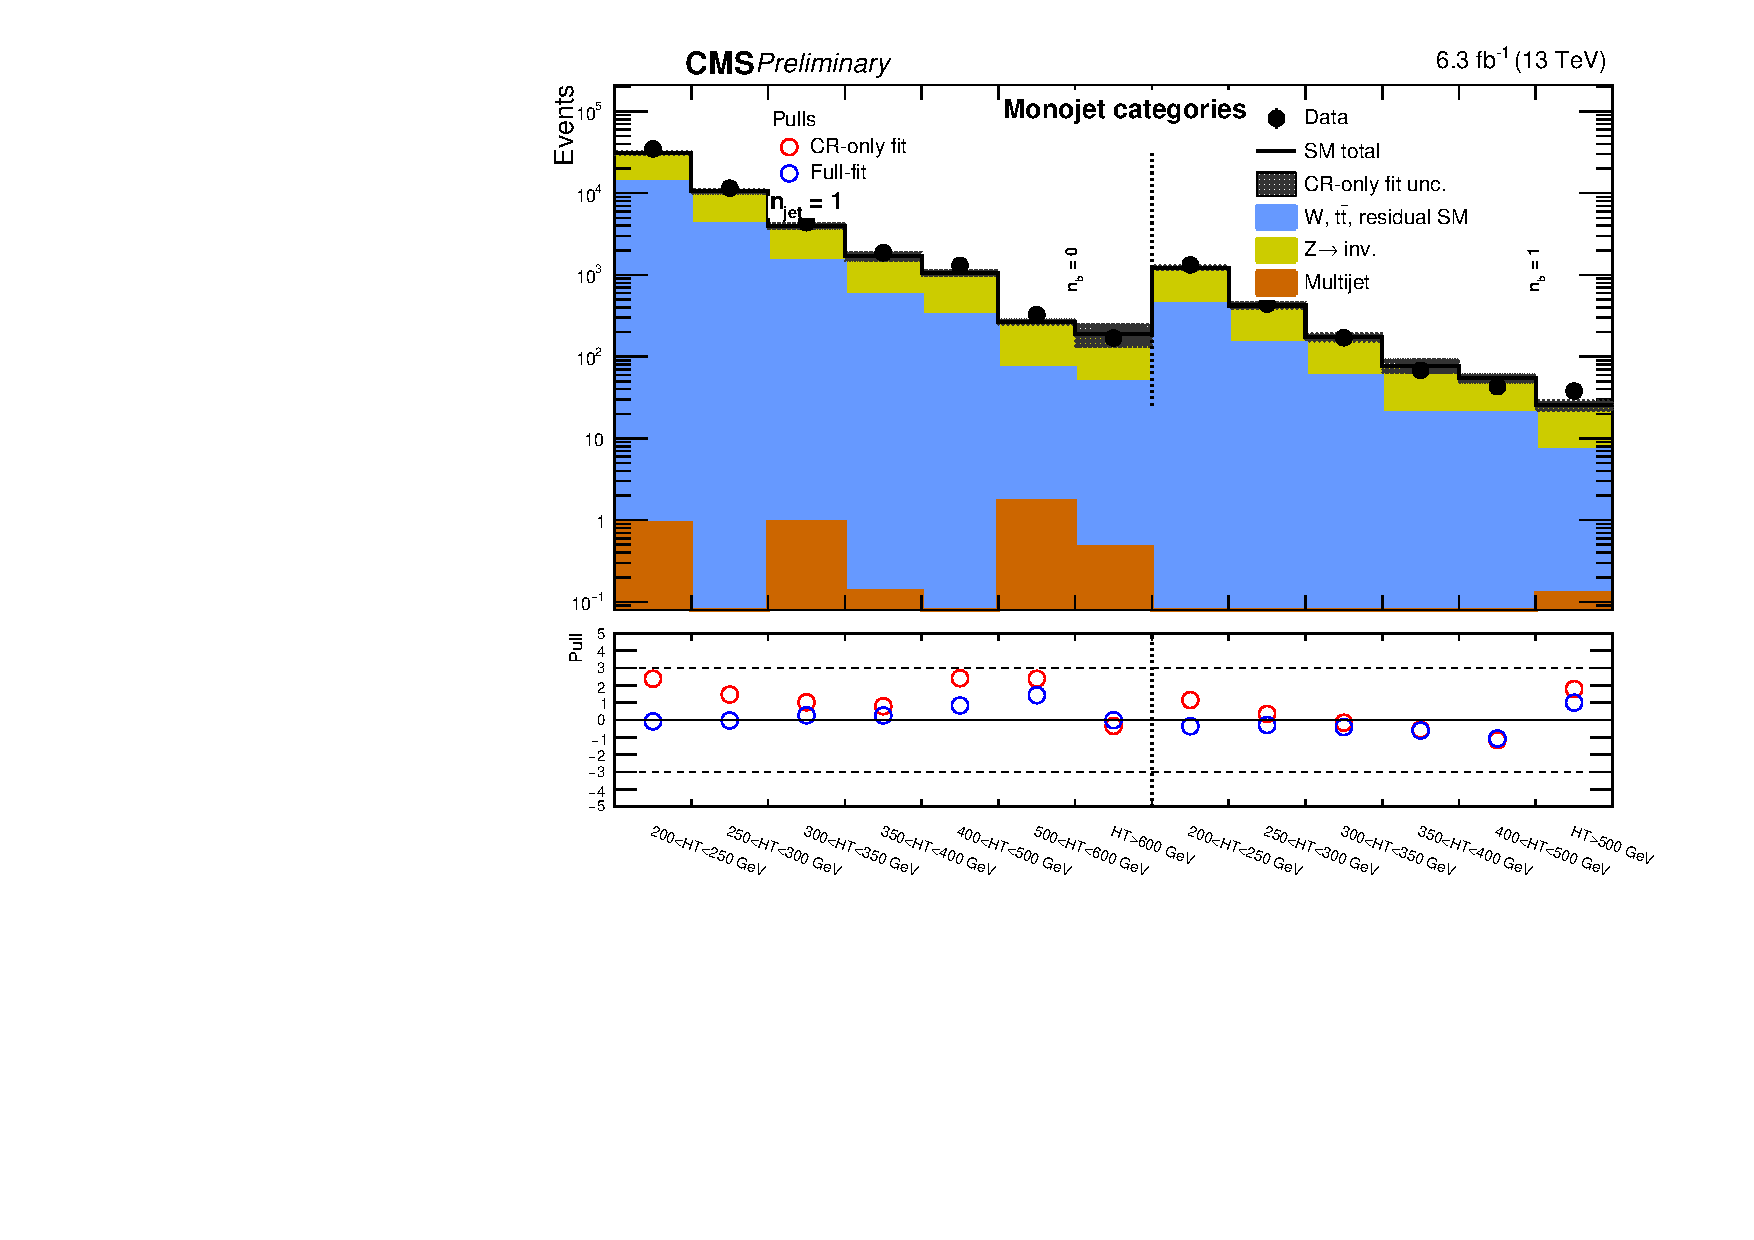
\includegraphics[width=0.7\textwidth]{summaryPlot_Monojet_prefit_overlay_fit_b_CRFit}
    \caption{(Top panel) Event yields observed in data (solid circles)
      and SM expectations with their associated uncertainties (black
      histogram with shaded band) from a CR-only fit, integrated over
      \HTmiss, as a function of \nb, and \scalht for the monojet
      category ($\njet = 1$) in the signal region. (Bottom panel). The
      significance of deviations observed in data with respect to the
      SM expectations from the CR-only (red circles) and full fit
      (blue circles).  }
    \label{fig:mono}
  \end{center}
\end{figure}

\begin{figure*}[!h]
  \begin{center}
    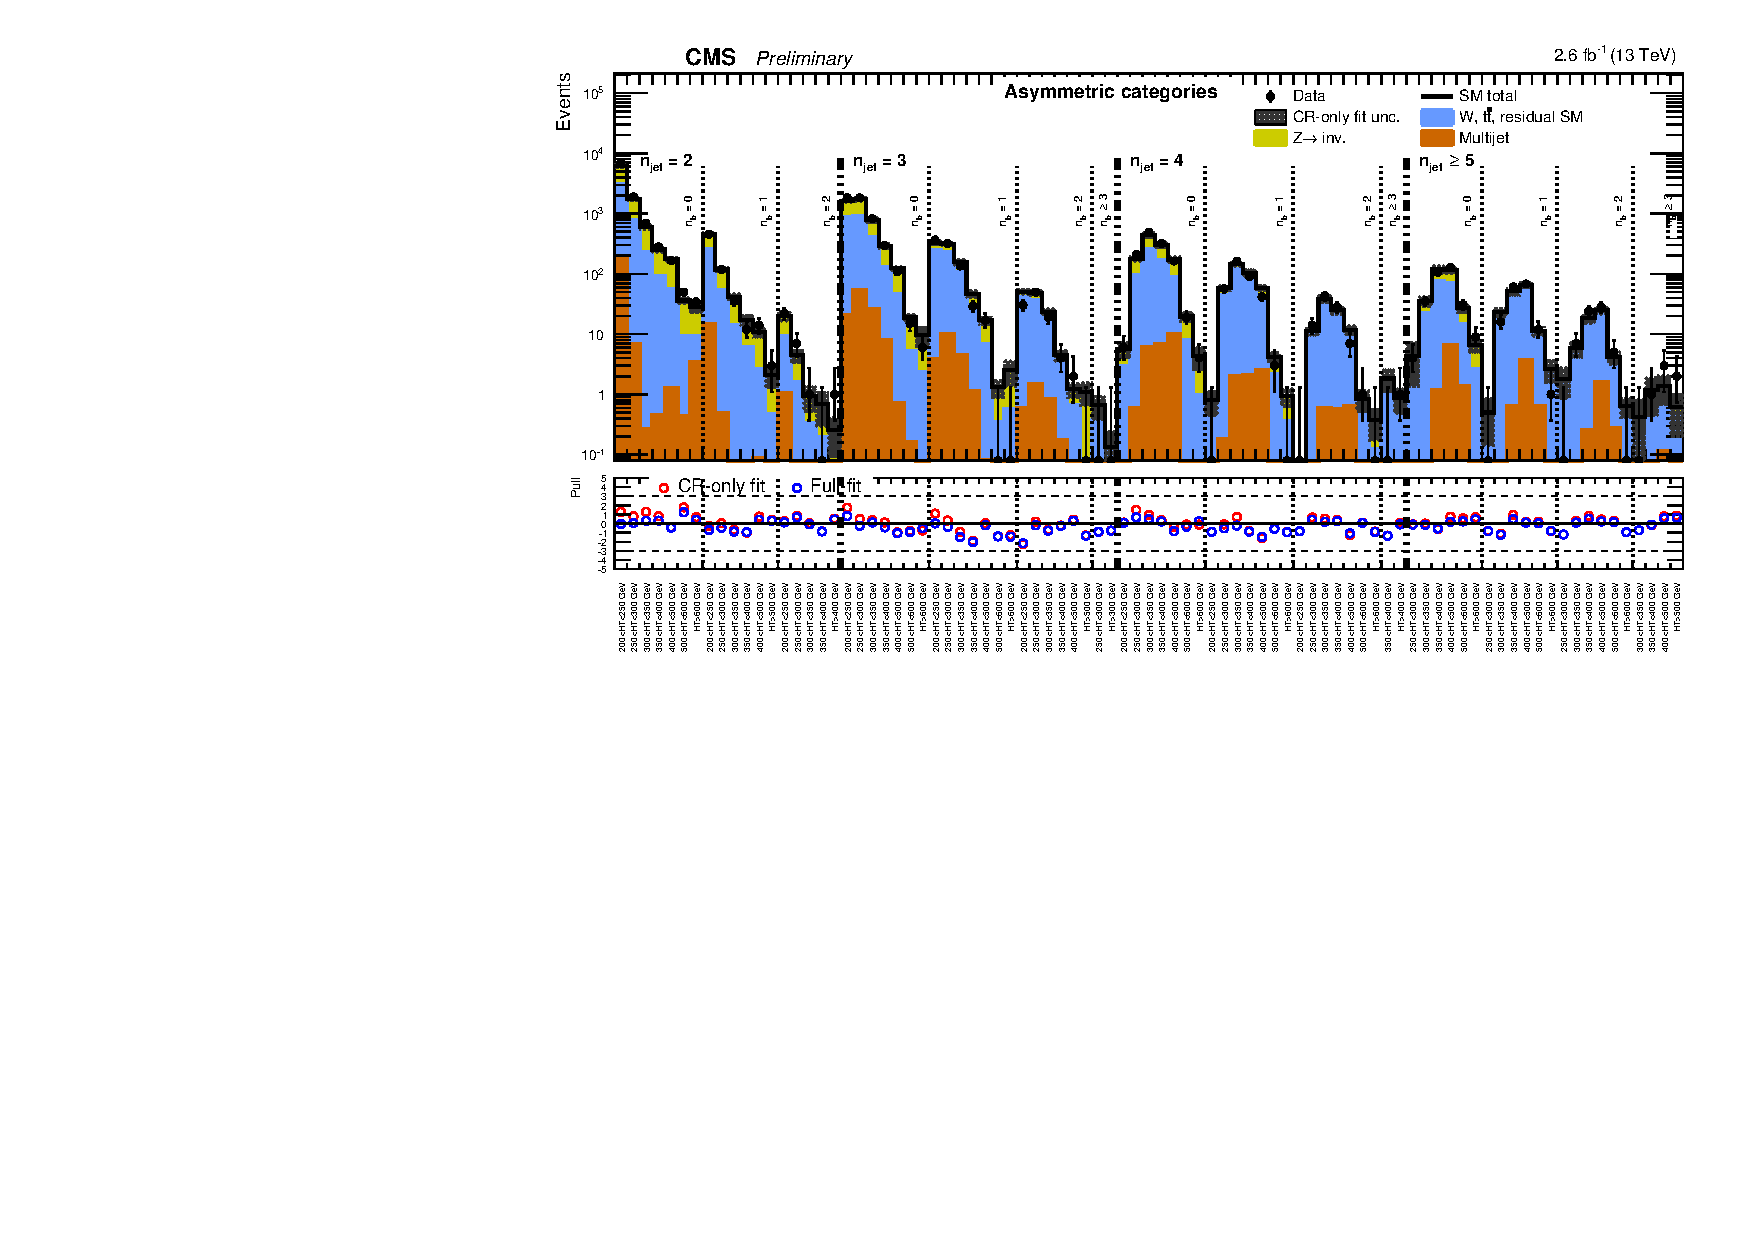
\includegraphics[angle=90,width=0.7\textwidth]{summaryPlot_Asymmetric_prefit_overlay_fit_b_CRFit}
    \caption{(Top panel) Event yields observed in data (solid circles)
      and SM expectations with their associated uncertainties (black
      histogram with shaded band) from a CR-only fit, integrated
      over \HTmiss, as a function of \njet, \nb, and \scalht for the
      ``asymmetric'' \njet categories in the signal region. (Bottom
      panel). The significance of deviations observed in data with
      respect to the SM expectations from the CR-only (red circles)
      and full fit (blue circles).  }
    \label{fig:asym}
  \end{center}
\end{figure*}

\begin{figure*}[!h]
  \begin{center}
    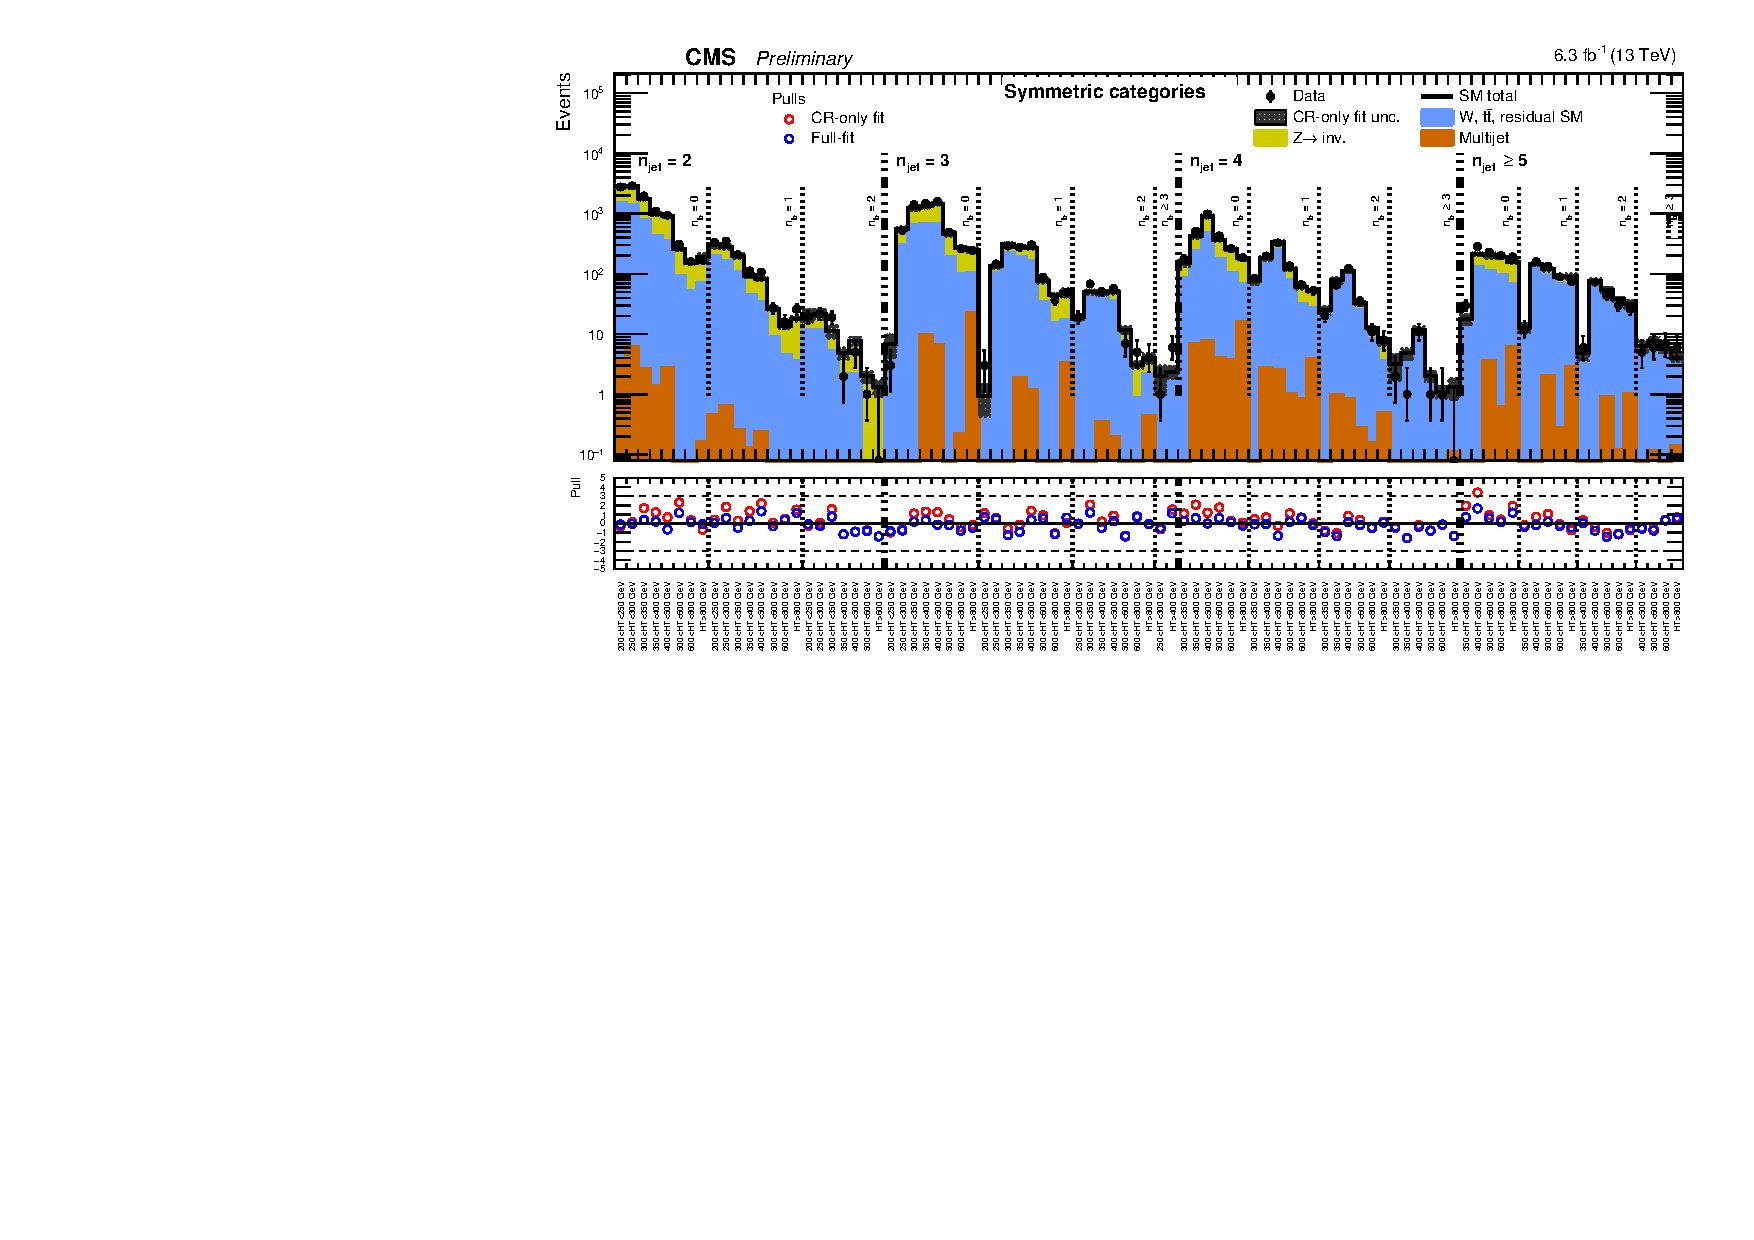
\includegraphics[angle=90,width=0.7\textwidth]{summaryPlot_Symmetric_prefit_overlay_fit_b_CRFit}
    \caption{(Top panel) Event yields observed in data (solid circles)
      and SM expectations with their associated uncertainties (black
      histogram with shaded band) from a CR-only fit, integrated over
      \HTmiss, as a function of \njet, \nb, and \scalht for the
      ``symmetric'' \njet categories in the signal region. (Bottom
      panel). The significance of deviations observed in data with
      respect to the SM expectations from the CR-only (red circles)
      and full fit (blue circles).  }
    \label{fig:sym}
  \end{center}
\end{figure*}

\begin{figure*}[tbhp]
  \begin{center}
    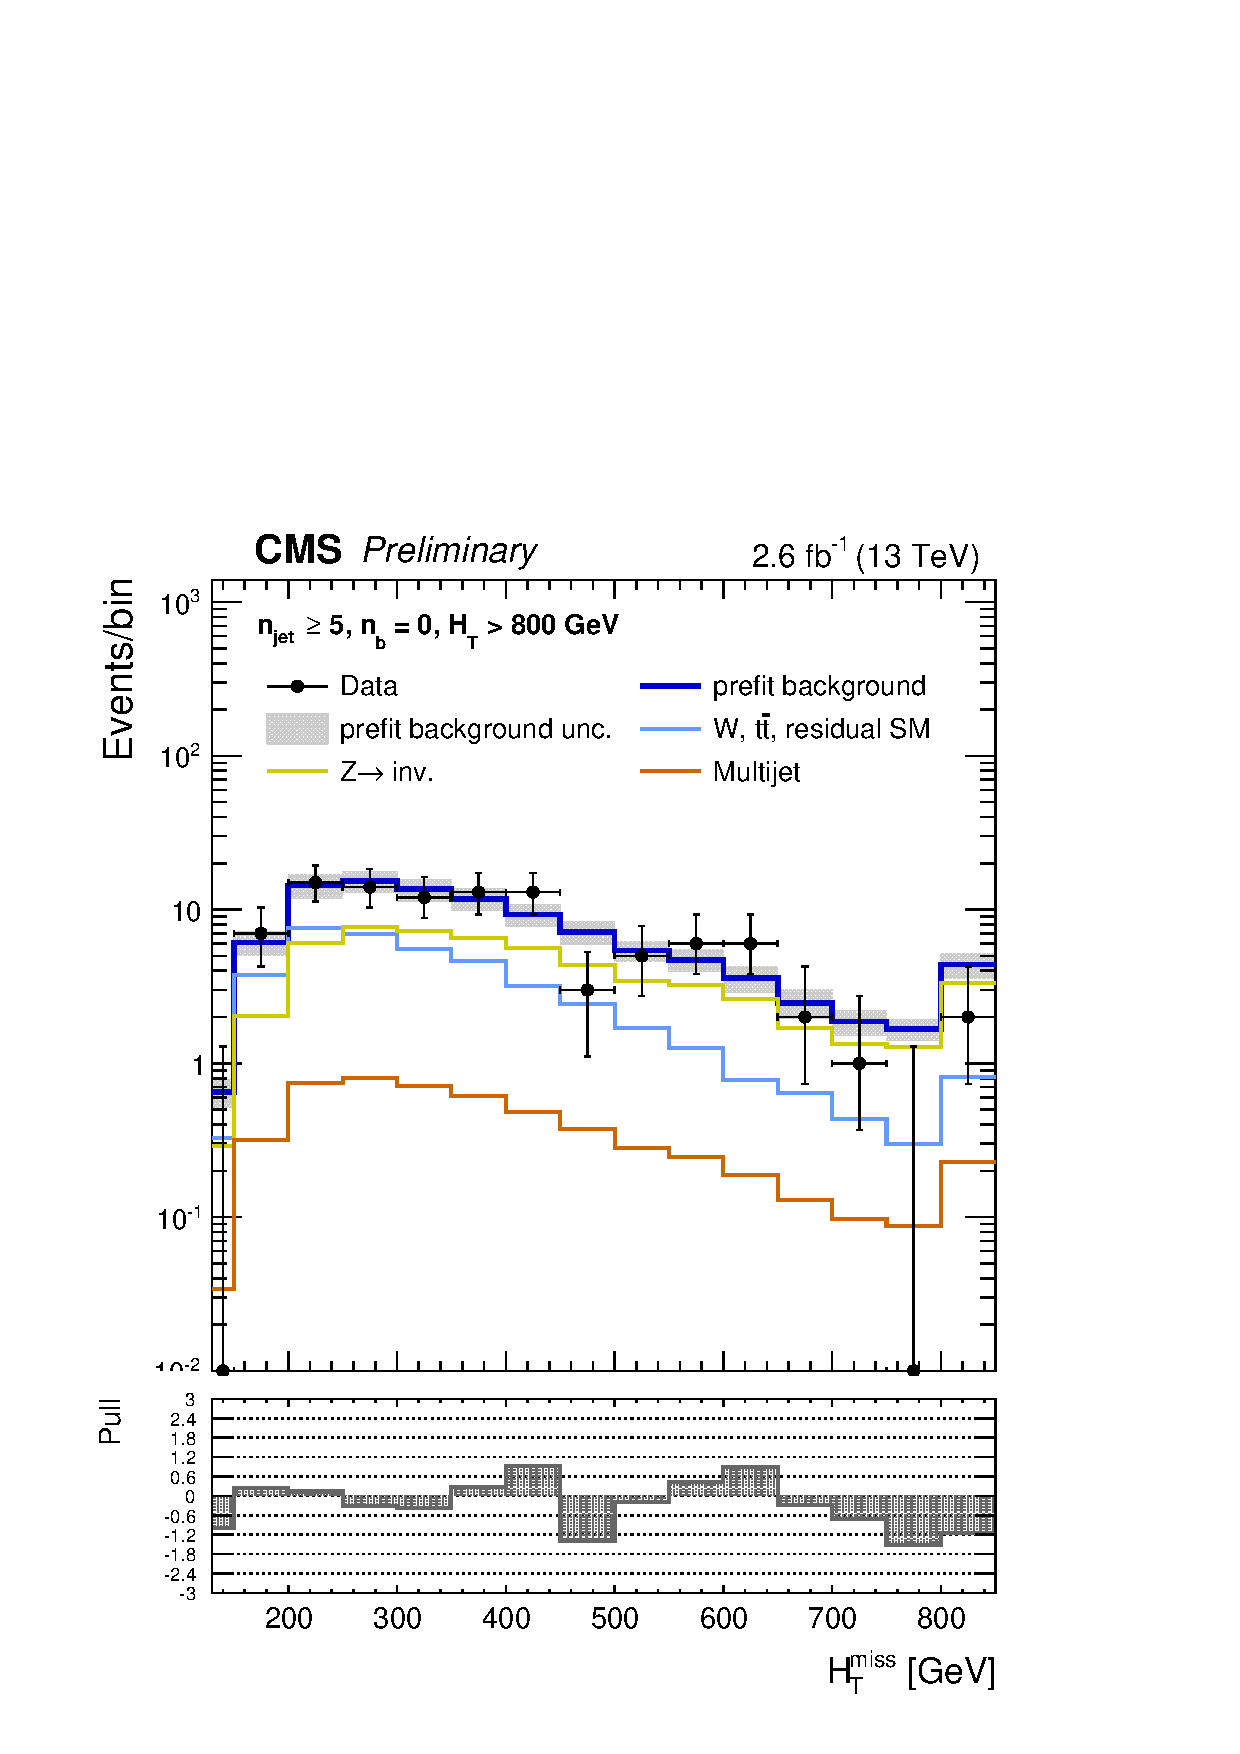
\includegraphics[width=0.6\textwidth]{mhtShape_eq0b_ge5j_800_Inf_prefit.pdf} 
    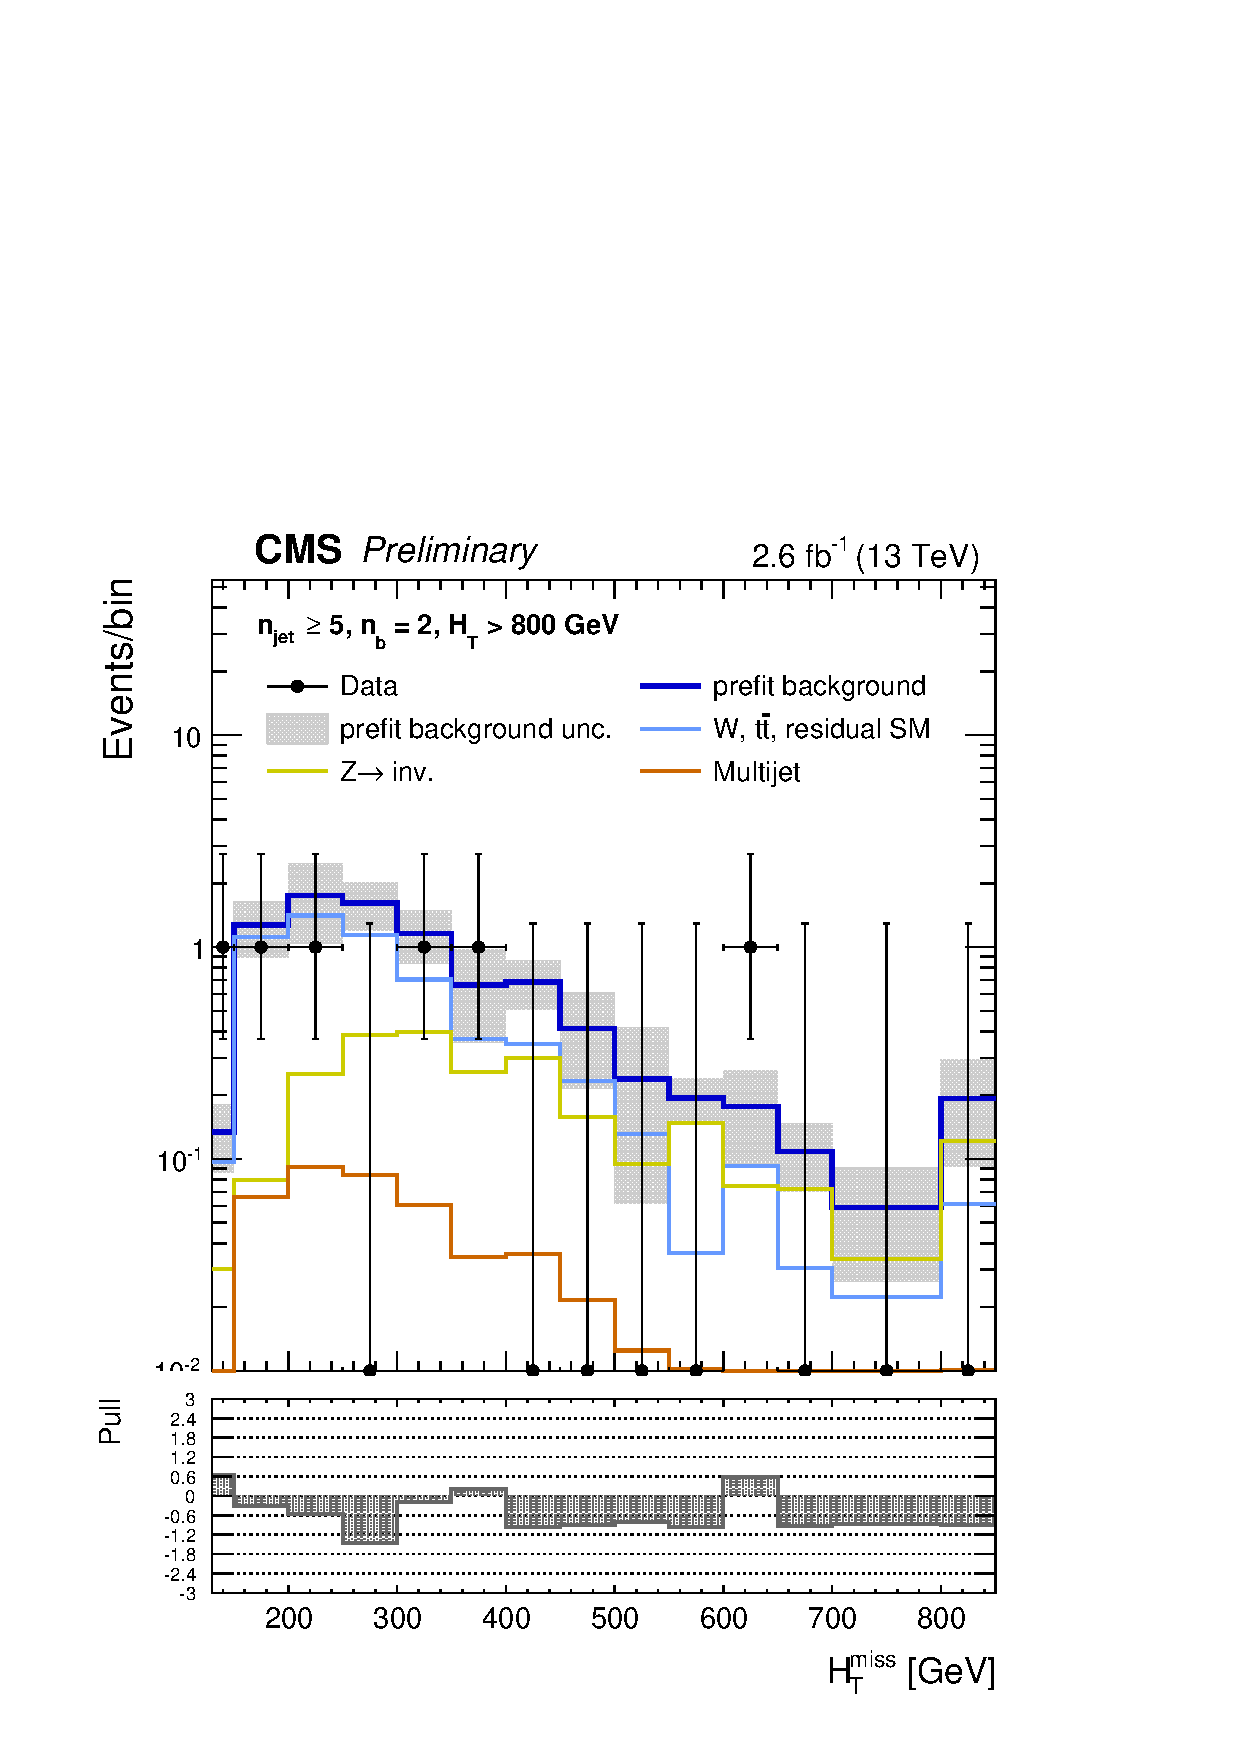
\includegraphics[width=0.6\textwidth]{mhtShape_eq2b_ge5j_800_Inf_prefit.pdf} \\
  \end{center}
  \caption{ The \mht distribution observed in data and the expected
    distribution for the sum of all SM background processes in two
    representative event categories at high \njet and \scalht. 
    \label{fig:mht-templates} }
\end{figure*}

%%__________________________________________________________________||
\clearpage
\section{Interpretation}

The results of this search are interpreted in terms of upper limits in
the production cross section as a function of the parent sparticle and
LSP mass for simplified models~\cite{Alwall:2008ag, Alwall:2008va,
  sms} that represent the pair production of gluinos and their
subsequent decays to four quarks and two LSPs. The event samples for
the simplified models are generated with \MADGRAPH V5~\cite{madgraph}.
Inclusive, process-dependent, NLO calculations of SUSY production
cross sections, with next-to-leading-logarithmic (NLL) corrections,
are obtained with the program \PROSPINO~\cite{Beenakker:1996ch,
  PhysRevD.80.095004,PhysRevLett.102.111802, PhysRevD.80.095004,
  1126-6708-2009-12-041, doi:10.1142/S0217751X11053560,
  susy-nlo-nll}. The samples are generated using the
CTEQ6L1~\cite{Pumplin:2002vw} PDFs. The distribution of the number of
pp interactions per bunch crossing for the simulated samples matches
that observed in data. Various uncertainties in the experimental
acceptance are considered, for which typical magnitudes \fixme{\it
  will be summarised}. 
%are summarised in Table~\ref{tab:signal_systs}.

%\begin{table}[h!]
%  \caption{%CMS {\it Simulation}. 
%    Typical magnitudes of systematic uncertainties in the experimental
%    acceptance for the signal models considered.
%  }
%  \label{tab:signal_systs}
%  \centering
%  \footnotesize
%  \begin{tabular}{ lccc }
%    \hline
%    \hline
%    Systematic source              & Type          & Correlated & Typical magnitude (\%) \\
%    \hline
%    Luminosity                     & Normalisation & Yes        & 4.6                    \\
%    Monte Carlo statistics         & Norm. + shape & No         & 1--50                  \\
%    Initial state radiation        & Norm. + shape & Yes        & 0--30                  \\
%    Jet energy scale               & Norm. + shape & Yes        & 3--10                  \\
%    Pile-up                        & Norm. + shape & Yes        & 0-5                    \\
%    Trigger                        & Norm. + shape & Yes        & 0--10                  \\
%    Parton density functions       & Normalisation & No         & 10                     \\
%%    Renormalisation/factorisation & Norm. + shape & No         & 10                     \\
%    b-tag scale factors            & Norm. + shape & Yes        & 5--30                  \\
%    Lepton scale factors           & Normalisation & Yes        & $<$5                   \\
%    \hline
%    \hline
%  \end{tabular}
%\end{table}
  
%\begin{figure*}[thp!]
%  \begin{center}
%    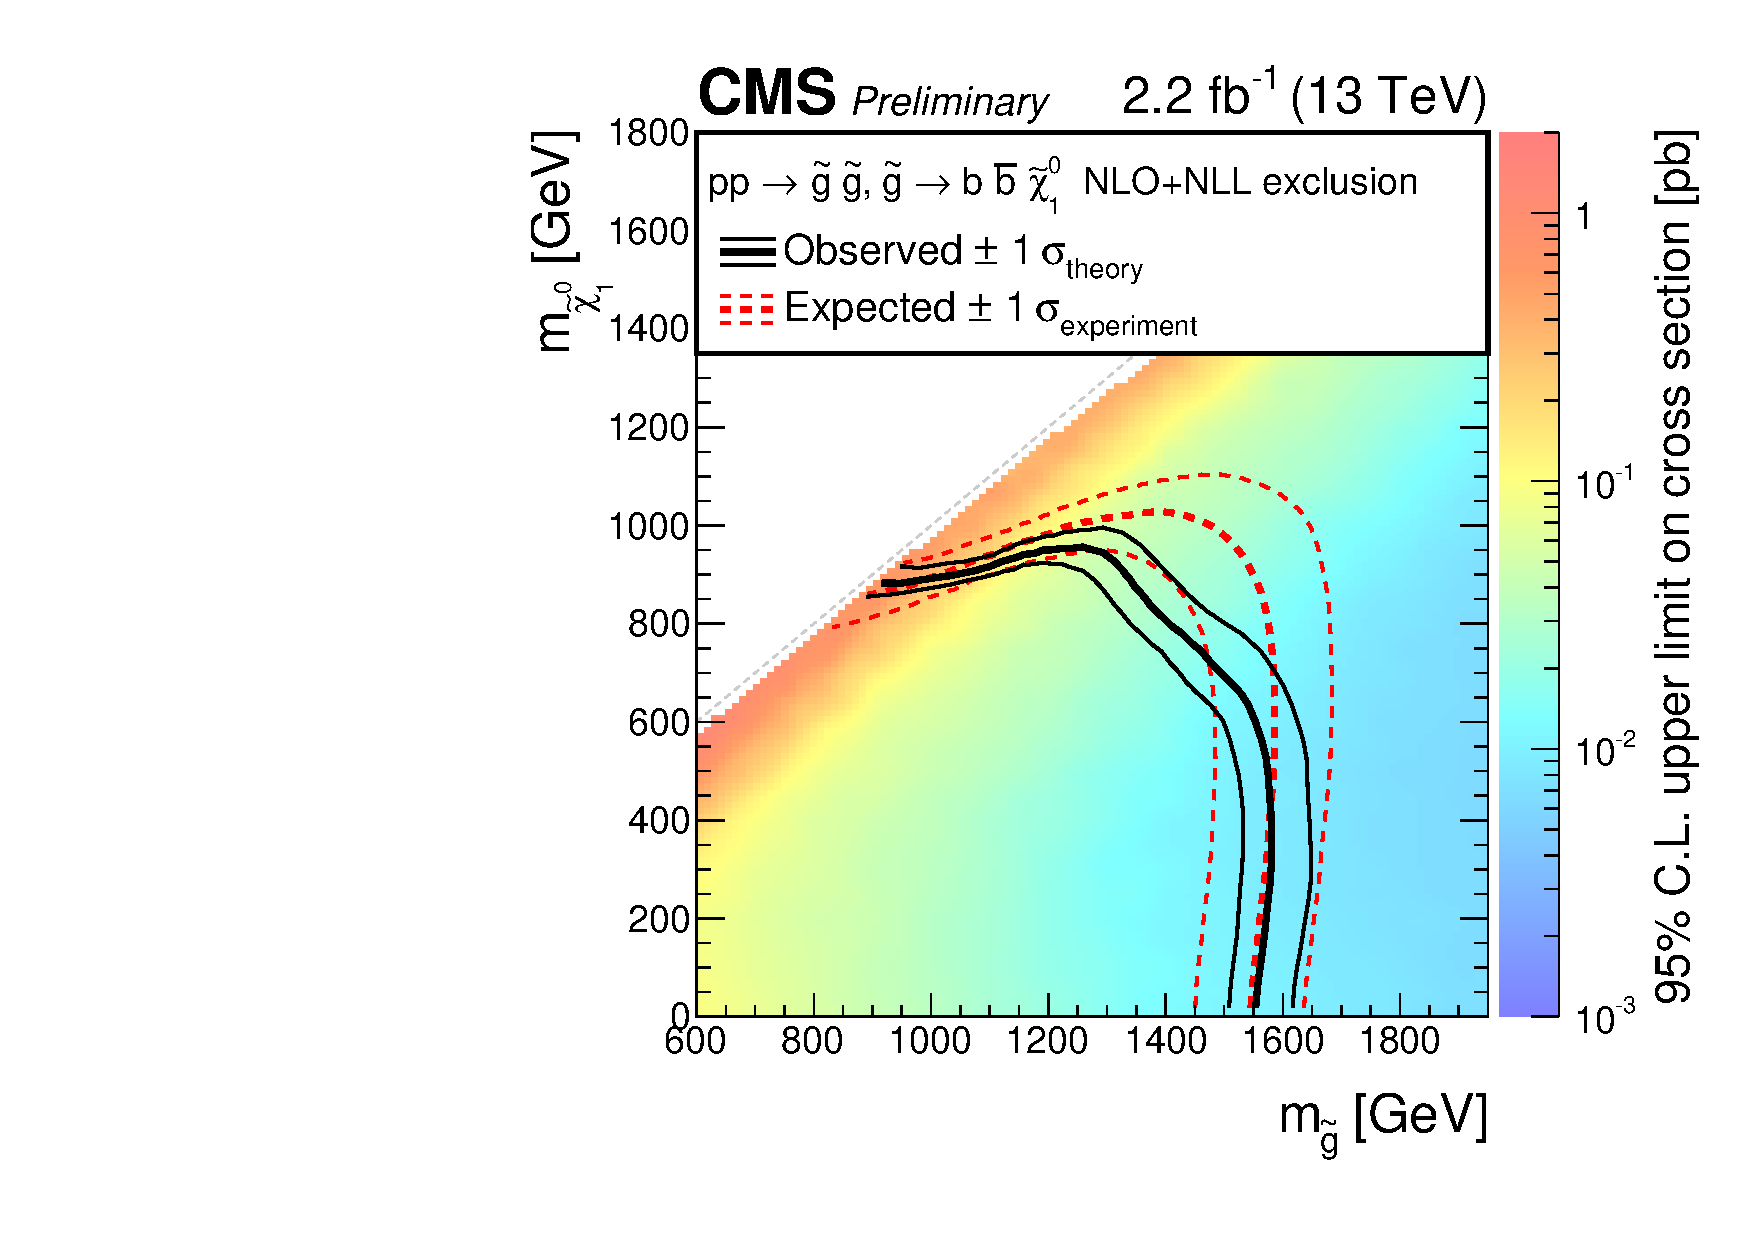
\includegraphics[width=0.49\textwidth]{t1bbbbRA1XSEC.pdf} \,
%    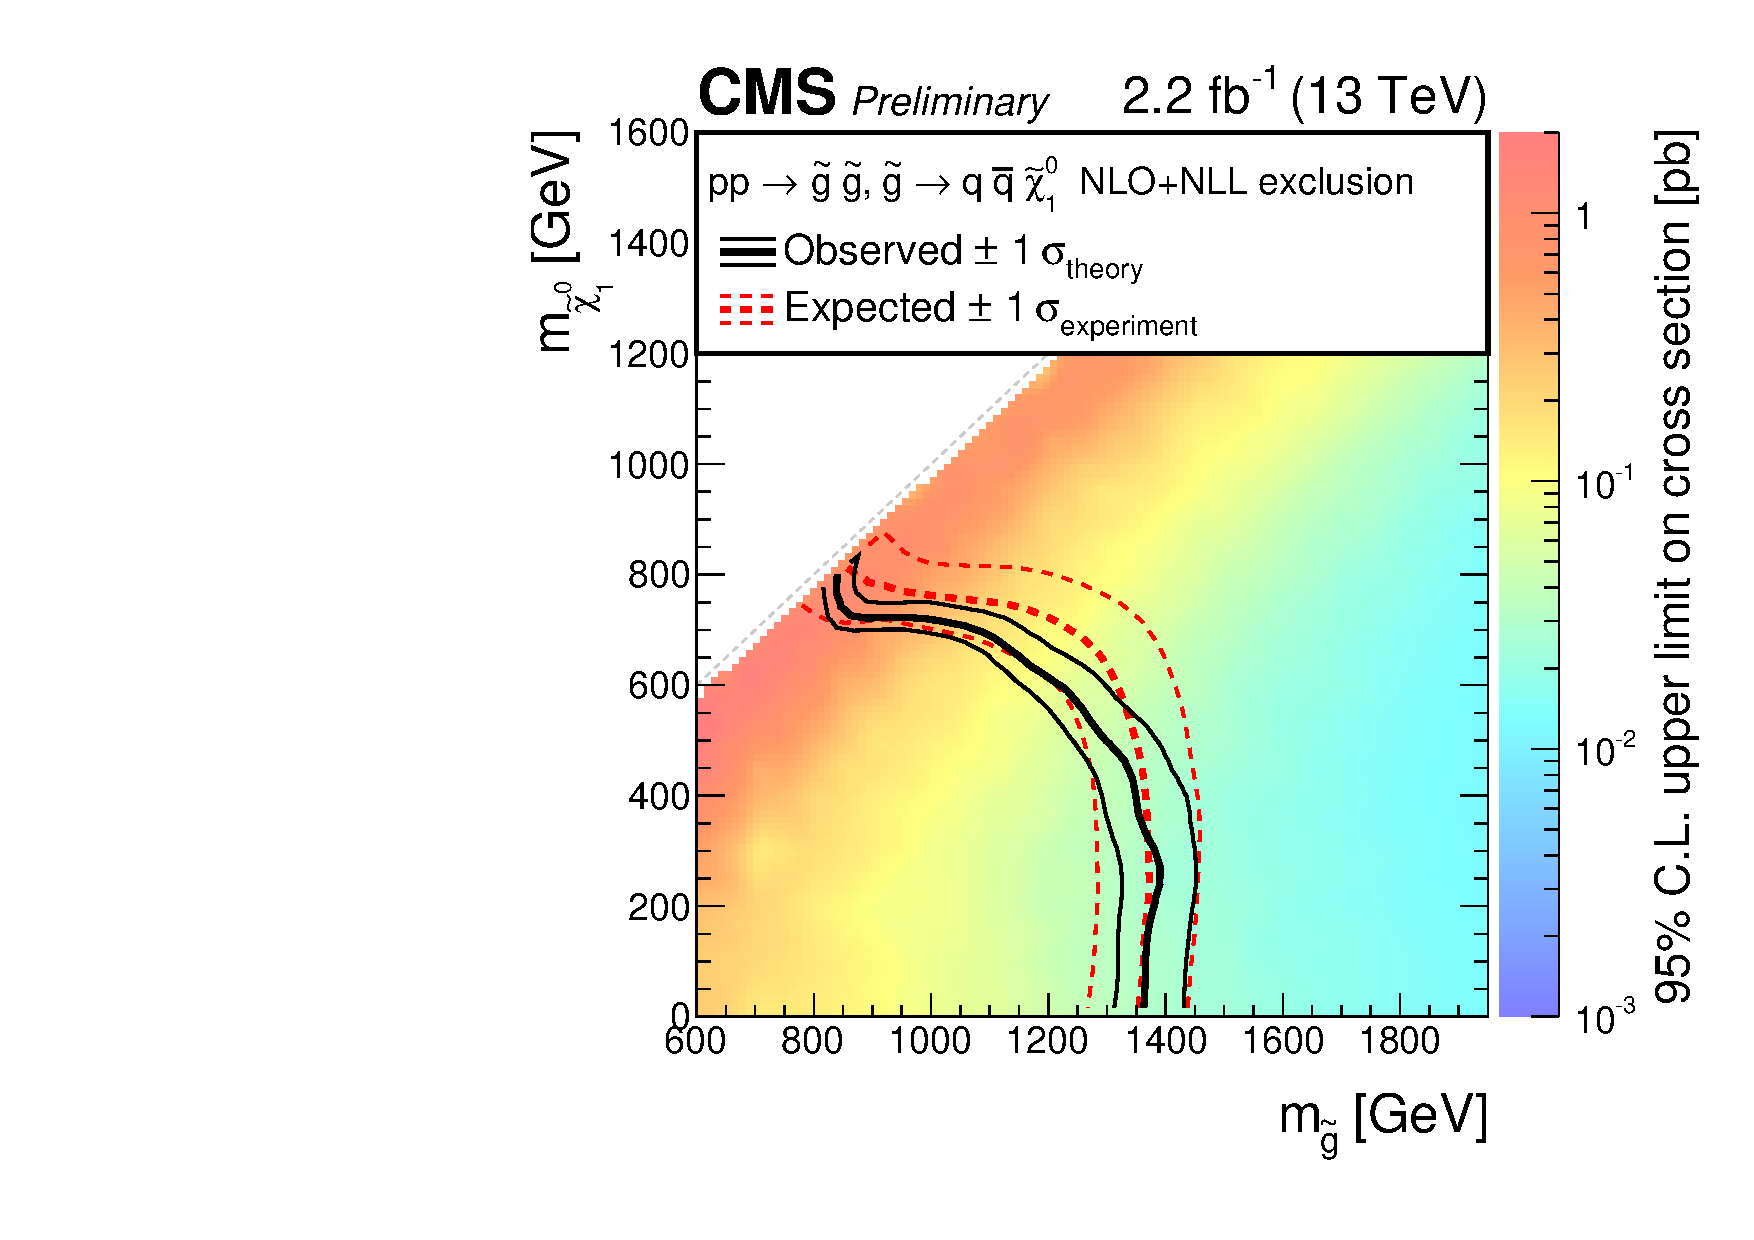
\includegraphics[width=0.49\textwidth]{t1qqqqRA1XSEC.pdf} \\
%    \caption{Observed upper limit in cross section at 95\% CL
%      (indicated by the colour scale) for simplified models that
%      assume the pair production of gluinos, as a function of the
%      gluino and $\chiz_{1}$ masses for gluino three-body decays to
%      $b\bar{b}\chiz_{1}$ (left) and $q\bar{q}\chiz_{1}$ (right). The
%      black solid thick (thin) line indicates the observed mass
%      exclusion region assuming the nominal (${\pm}1 \sigma$ theory
%      uncertainty) production cross section. The red dashed thick
%      (thin) line indicates the median (${\pm}1 \sigma$ experimental
%      uncertainty) expected exclusion.
%      \label{fig:limits-sms} }
%  \end{center}
%\end{figure*}

Figure~X \fixme{\it will show} 
%\ref{fig:limits-sms} shows 
the observed upper limit on the
production cross section at 95\% confidence level (CL) as a function
of the gluino and LSP masses for a range of simplified models assuming
pair production of gluinos. The observed excluded regions are
determined for gluino pair production assuming decoupled squarks. Also
shown are the observed excluded regions when varying the production
cross section by its theoretical uncertainty, and the expected
excluded region with the ${\pm}1$ standard-deviation ($\sigma$)
variations. The search places stringent limits in the mass parameter
space, with observed exclusions in gluino and LSP masses as high as
$\sim$X\gev and $\sim$Y\gev, respectively.

%%__________________________________________________________________||
